\documentclass[a4paper, 11pt, twocolumn]{article}
\usepackage{caption}
\usepackage{graphicx}
\usepackage{color} %colors in text
\usepackage{textcomp} % 
\usepackage[T1]{pbsi} %hand writting nice 
\usepackage[T1]{fontenc} %more fonts
\usepackage{mathrsfs} % letters for math
\usepackage{fullpage} % no margins
\usepackage{amsmath} % math formulas
\usepackage[all]{xy} % for drawing
\usepackage{listings}
\usepackage{algorithmic}
\usepackage{algorithm}
\usepackage{amssymb}
\usepackage[parfill]{parskip}
\definecolor{gray}{rgb}{0.7,0.7,0.7} 
\usepackage{enumerate} %for enumerate
\newcommand{\ds}{\displaystyle}
\newcommand{\todo}[1]{\textcolor{red}{\textbf{#1}}}
\newcommand{\fade}[1]{\textcolor{gray}{\textbf{#1}}}
\date{} % no date
\author{\fade{Nimrod Raiman [0336696]}\\\fade{Silvia L. Pintea [6109960]}}
\title{Rock, Paper \& Scissors with Nao}
\begin{document}
    \maketitle
	%ABSTRACT SECTION__________________________________________
    \abstract{Throughout this paper we are going to explain our work on teaching a humanoid robot (\emph{Nao}) to play \emph{"Rock, paper \& scissors"}. In order to accomplish this task we have used different theoretical methods which are described in the section~\ref{sec:methods}. In Section~\ref{sec:results} are presented our experimental results. Finally, we give an overall view of this paper and indicate the possible future work that could be done on this subject.}  
	%SECTION SECTION_________________________________________
    \section{Introduction}
	\label{sec:intro}
        \emph{"Rock, Paper \& Scissors"} is an easy and well known game. This is the reason for which it is interesting to learn a robot how to play it against human players. In order to do that the robot needs to be able to recognize the hands of its opponent and classify the gesture as: \emph{"rock"}, \emph{"paper"} or \emph{"scissors"}.\\	
		\hspace*{10px}In this paper we describe our approach to accomplish this in real time. Our solution is fairly robust to lightning condition and also the gestures of the player need not be restricted to certain angles or positions in the frame (given that the gesture is clear enough).\\ 
        \hspace*{10px}Our problem has been split into three main tasks: extracting the hands from the webcam stream, recognizing the gesture of the extracted hand and implementing motion and speech on \emph{Nao}. Throughout our project we have tried different approaches in order to find the best method to solve the problem.\\
		 \hspace*{10px}We have experimented with methods such as: \emph{backprojection of probability histogram} for hand detection, \emph{Gabor filters} and \emph{PCA} for feature extraction.\\
		 \hspace*{10px}We will start by describing the methods that we have tried and then continue by giving an overview of the results and the conclusions.   
	%METHODS SECTION__________________________________ 
    \section{Methods}
	\label{sec:methods}
		For hand detection and recognition we have employed two different techniques: a naive approach and the backproject of the probability histogram of the pixels corresponding to skin.\\
		\hspace*{10px}For the gesture recognition we have experimented with different sets of data and we have extracted different features using methods such as: \emph{PCA} and \emph{Gabor filters}. We have also tried using two different types of classifiers: \emph{SVM} (support vector machine) and \emph{Knn} (K nearest neighbors).\\
		\hspace*{10px}We will continue by giving a more detailed description of the methods employed. 
        \subsection{Hands extraction}
		\label{sec:Meth_exrctHands}
        \subsubsection{Naive approach}
		 Our first approach for extracting the area from the webcam stream that corresponds to the hand was to define thresholds for the hue and the saturation values for the frames received from the webcam. The resulting binary image would contain all pixels corresponding to skin. Then using erosion and dilation noise was reduced. From the resulting binary image we then could easily find the area corresponding to the hand.\\
       	\hspace*{10px}This naive approach was not reliable enough because it is very sensitive to objects with a color that is close to skin color in the view of the camera. This approach is also very sensitive to lightning changes (artificial light is more blue than sunlight). Finally, the thresholds need to be defined very broad to make this work for the majority of skin colors -- fact which might introduce even more false skin responses.        
		\subsubsection{Backprojection of skin pixels}
       	After realizing that our first approach was too naive and instable we needed to create a more robust skin finder.\\
       \hspace*{10px} Inspired by \cite{IMS} and \emph{Gijs Molenaar} we implemented a skin \emph{PDF} (probability distribution function) approach. In order to make such a \emph{PDF} we needed to build a histogram (normalizing the histogram would give a \emph{PDF}) of an area that we knew for sure it was representative for the skin color of the person standing in front of the camera. For this we chose to use the face area. Using a frontal face \emph{Haar detector} we were able to find the face of the person standing in front of the camera and we constructed a histogram from the inside area of the rectangle returned by the face detector. We removed the borders in order to loose as much background and hair as possible and get an even more reliable skin \emph{PDF}.\\
       \hspace*{10px} Once we had the histogram, we could backproject it on the image. The resulting image was a gray-scale one showing what areas are more or less probable to correspond to skin (see Figure \ref{img:skinProb} -- left image). We first set the probability of the pixels in the face area to zero, because we did not want this to be interfering with finding the hand in the frame. Then we thresholded this image to get rid of areas with very low probability for the skin. Using rough erosion and dilation we got rid of noise and connected the areas that belonged together. This was done roughly because at this step, we just wanted to find the area of the hand and process it separately in a more sophisticated manner. From the image obtained in this manner we have selected the biggest blob of pixels that were connected and chose this as the most probable area to correspond to the hand.\\
       \hspace*{10px}Once we had the area that corresponded to the hand, we went back to the backprojection image. Here we selected the hand area again to do a more sophisticated thresholding, erosion and dilation on it. After dilation a part of the hand area would end up being white -- corresponding probably to the skin, and another part being black -- probably not skin. The black area was left unchanged while the white area was replaced by the original gray-scale image. The final step was to resize the hand image to \emph{$70\times 70$} pixels to match the training images.\\
		\begin{figure}[!hbtp]
		   \centering
		   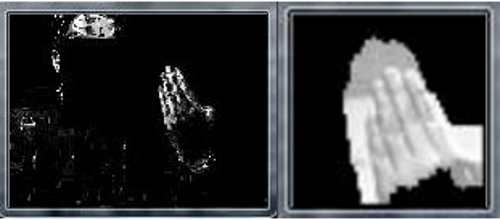
\includegraphics[width=0.5\textwidth]{hands.png}
			\caption{Hand detection -- Example}
			\label{img:skinProb}
	   	\end{figure}	
		\hspace*{10px}The resulting image was one in which the hand area was selected and most of the background was removed (see Figure \ref{img:skinProb} -- right image).
		%GESTURE RECOGNITION______________________________________________
        \subsection{Gesture recognition}
		For the gesture recognition task we have started by using a training set containing images of hands of \emph{$70\times 70$}px with different backgrounds. The problem proved to be too complex for our classifiers so we have decided to switch to a simpler one which would contain only centered hands and a black background.\\ 
		\hspace*{10px}Out of this dataset we have extracted the features to be used during the classification.
		\label{sec:Meth_clssifyHands}
		\subsubsection{PCA}
		The first technique we have tried was \emph{PCA}. We have computed the \emph{eigen-hands} of our data and then we have projected each set, separately, on this space.\\
		\hspace*{10px}There are three steps for generating the \emph{eigen-hands}:
		\begin{itemize}
		\item Subtracting the mean of the data
		\item Computing the covariance of the data and the eigenvectors of the covariance matrix
		\item Projecting each training set (corresponding to each sign: \emph{"rock"}, \emph{"paper"} or \emph{"scissors"}) on the space defined by the eigenvectors
		\end{itemize}
		\hspace*{10px}For high-dimensional data a better approach than computing the eigenvectors of the matrix: \emph{$Data^T \times Data$} (which for a dataset of \emph{[N,D]} with \emph{$D\gg N$} has the dimension \emph{[D,D]}) would be to use an intermediate step and compute the eigenvectors \emph{$V \rightarrow eigh(Data\times Data^T)$} and then determine the final \emph{eigen-space}: \emph{$U \rightarrow \frac{Data^T\times V}{norm(Data^T\times V)}$}.\\
		\hspace*{10px}Unfortunately, given the fact that \emph{PCA} is not background invariant, translation invariant or rotation invariant the results were not as good as we were expecting.	
		\subsubsection{Gabor filters}
		The next technique that we have attempted to use for the feature extraction part was: \emph{Gabor wavelets}.\\
		A \emph{Gabor wavelet} is created by defining the size of the wavelet to be generated and then by looping over the coordinates of each pixel (\emph{x} and \emph{y}) and applying the following formula:\\
		\begin{table}[!htbp]
		\begin{tabular}{| c |}
			\hline\\
			\fontfamily{cmbr}\selectfont\scriptsize
	 		\textbf{$\text{g(x, y, $\lambda$, $\theta$, $\psi$, $\sigma$, $\gamma$) = exp(- $\frac{x\prime^2+\gamma^2y\prime^2}{2\sigma^2}$) cos(2$\Pi$ $\frac{x\prime}{\lambda}$ + $\psi$)} $}\\[15px]
			\fontfamily{cmbr}\selectfont\small
			where $x\prime$ = x cos$\theta$+y sin$\theta$\\[2px]
			\fontfamily{ptm}\selectfont\small
			and $y\prime$ = -x sin$\theta$+y cos$\theta$\\[2px]
			\hline
		\end{tabular}
		\end{table}

		The parameter $\lambda$ represents the frequency of the stripes in the wavelet, $\theta$ gives the angle of the stripes, $\psi$ is a translation parameter, $\sigma$ gives the size of the stripes while $\gamma$ indicates how elliptical they are.\\  
		\begin{figure}[!hbtp]
		   \centering
		   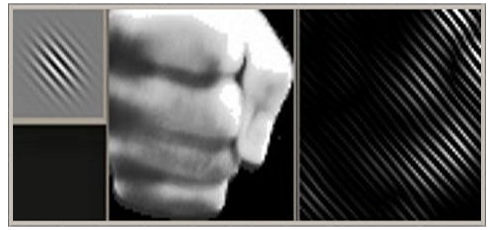
\includegraphics[width=0.5\textwidth]{gabor.png}
			\caption{Gabor wavelet Example}
	   	\end{figure}	
		\hspace*{10px}Each image in the training set was convolved with the \emph{Gabor wavelets} and then reshaped as a single row.\\
		\hspace*{10px}In our project we have used 4 \emph{Gabor wavelets} (with the angle $\theta \in \{0, \frac{\Pi}{4}, \frac{\Pi}{2}, \frac{3\Pi}{4}\}$). Each image was convolved with each one of these 4 wavelets and then reshaped as a row. All 4 results obtained in this manner were then concatenated and stored in single row for each image.\\
		\hspace*{10px}Besides using these 4 \emph{Gabor wavelets} we have also tried concatenating to the result the original image also reshaped on a single row.\\
		\hspace*{10px}Unlike the \emph{PCA}, this method gave satisfactory results, fact which indicates that it is capable of determining a set of representative features of our training set.
		\subsubsection{Classification}
		In order to be able to classify the gesture we have tried using both the \textbf{SVM} (support vector machine) and \textbf{Knn} (K nearest neighbor) classifiers.\\
		\hspace*{10px}Given the fact that the data is not perfectly aligned (hands have slightly different positions in the image and different angles) the problem seemed to be too hard for the \textbf{SVM}. It was not able to find a good boundary between the classes.\\
		\hspace*{10px}To ensure that our approach was correctly implemented we have created a more aligned training set (the hands had only small differences in the angles of their orientation $ \in [-20, +20]$ degrees). For this task the \textbf{SVM} classifier was able to perfectly classify the data (it found a good boundary between the classes) and it gave an error of \emph{0.0}.\\
		\hspace*{10px}Because we did not want to restrict the player to only a small amount of positions and ways in which a sign could be made we have decided not to use \textbf{SVM}.\\
		\hspace*{10px}We have experimented also with the \textbf{Knn} classifier. This one was able to give accurate prediction even on the raw training images and thus we have decided to employ it for solving our task of gesture recognition.
		%NAO MOTION AND SPEECH________________________________________________________________
        \subsection{Motion \& Speech on Nao}
		\label{sec:Meth_naoPlay}
		\emph{Nao} is a humanoid robot with a processor of 500MhZ and 3 fingers that move simultaneously.\\
		\begin{figure}[!hbtp]
		 	\centering
			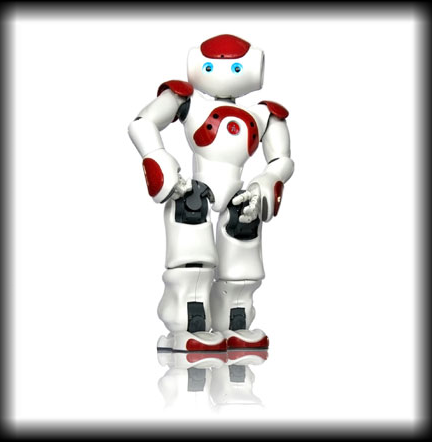
\includegraphics[width=0.45\textwidth]{Nao.png}
		 	\caption{Nao Aldebaran}
	   	\end{figure}			
		\hspace*{10px}Because of the limited computational power we had to run our software on a laptop that was connected to \emph{Nao}. All decisions were made by the software that was running on the laptop and the resulting interaction was sent and executed by \emph{Nao}.\\
		\hspace*{10px}Because the fingers can only be moved simultaneously we had to represent \emph{"paper"} as hand open, \emph{"rock"} as hand closed and \emph{"scissors"} by closing and opening the hand a few times.\\
		\hspace*{10px}In order to make \emph{Nao} move and talk we had to generate behavior files using the \emph{"Choregraphe"} simulator. These files were, then, transfered to \emph{Nao}\rq s memory and then we had to remotely connect to \emph{Nao} using its \emph{IP} address and execute one of the predefined behaviors that was needed at that specific moment in the game.\\  
        \hspace*{10px}The hand-detection and gesture recognition parts needed to be run in parallel with \emph{Nao}\rq s motion and speech behaviors such that it would be able vocalize the outcome of the game by comparing it\rq s choice of move with the player\rq s one.
	%EXPERIMENTAL RESULTS SECTION_______________________________________ 
    \section{Results}
	\label{sec:results}
		We have trained our models using images of hands with different positions and orientations. We have used:
		\begin{itemize}
		\item \emph{1641} training examples for the \emph{"rock"} sign 
		\item \emph{1522} training examples for the \emph{"paper"} sign
		\item \emph{1377} training examples for the \emph{"scissors"} sign
		\end{itemize}
		The results are obtained using 50--fold cross validation.\\
		\begin{table}[!hbtp]
		\begin{tabular}{| c | c | c |}
			\hline\hline
			& & \\
			\textbf{Size} & \textbf{Method} & \textbf{Average Error}\\[5px] 
			\hline\hline
			  70$\times$70 & \emph{PCA} & 0.475\\
			\hline
			  20$\times$20 & \emph{PCA} & 0.470\\
			\hline
			  20$\times$20 & \emph{Gabor} & 0.021\\
			\hline
			  20$\times$20 & \emph{Gabor + PCA} & 0.510\\
			\hline
			  \textbf{20$\times$20} & \textbf{\emph{Gabor \& Image}} & \textbf{0.012}\\
		 	\hline
			  20$\times$20 & \emph{(Gabor \& Image)} & 0.447\\
		               & \emph {+ PCA}  &     \\ 			
			\hline
			  70$\times$70 & \emph{Grayscale} & 0.016\\
			\hline
			  20$\times$20 & \emph{Grayscale} & 0.014\\
			\hline
		\end{tabular}
		\caption{Average errors for different methods}
		\label{tab:res}
		\end{table}
		Besides using images of $70\times 70$ pixels we have also experimented with images scaled to $20 \times 20$ pixels. This idea proved to be a useful one because the slight difference in the positions of the hands in the images (the hands were not always centered) was considerably reduced and thus the need for translation invariant features was not as important as before. Also the fact that the images had smaller sizes has helped reduce the time required for the sign recognition.\\     
		\hspace*{10px}In Table~\ref{tab:res} are depicted the average errors we have obtained while testing our methods. We can notice from here that the \emph{PCA} tends to perform worst than the other methods. It can also be observed that the \emph{Gabor wavelets} have a high prediction accuracy and that the best results are obtained when concatenating the convolved images of \emph{Gabor wavelets} with the original image for the size of \emph{$20\times20$}px.  
	%CONCLUSIONS & FARTHER WORK SECTION________________________________
    \section{Conclusions}
	\label{sec:conclusion}
		Throughout this paper we have presented the methods we have employed in order to make a humanoid robot (\emph{Nao}) play \emph{"Rock, paper \& scissors"} against a human opponent.\\
 		\hspace*{10px}Our experiments indicate the fact that the \textbf{SVM} classifiers is not very well suited for solving this problem and that it is capable of finding a good boundary between the classes only in the case in which the orientation and the position of the hands does not vary too much. But on the other hand a more simple classifier like the \textbf{Knn} is capable of solving the problem and returning satisfactory results.\\
		\hspace*{10px}We have also seen that \textbf{PCA} was not able to give features strong enough to allow for a good classification performance. This might be due to the fact that \textbf{PCA} is not background invariant, rotation invariant or translation invariant.\\
		\hspace*{10px}Given the fact the the hand detection component of our project was not selecting hand as perfectly separated from the background as the ones used for training we had to enhance our training set with a number of examples given by the hand-detection component in order to ensure stability to our system and a more precise and robust prediction.\\
		\hspace*{10px}In the present our software runs at a rate of 4 frames per second. With some proper optimization techniques this can be improved to make \emph{Nao} react even faster and more naturally.\\
		\hspace*{10px}Finally, we believe that other methods might give results as good as the ones presented here. Probably a good idea would be to try employing \emph{SIFT} features in solving this problem.
    %BIBLIOGRAPHY SECTION______________________________________________
	\begin{thebibliography}{2}
		\bibitem{gwenns}
		Yen-Ting Chen, Kuo-Tsung Tsen, \emph{Developing a Multiple-angle Hand Gesture Recognition System for Human Machine Interaction}; 2007
		\bibitem{gabor}
		M. R. Tuner, \emph{Texture Discrimination by Gabor Functions}; 1986, Biol. Cybern. 55, p. 71-82 
		\bibitem{IMS}
		Comaniciu, Dorin and Ramesh, Visvanathan and Meer, Peter, \emph{Kernel-Based Object Tracking}; 2003, IEEE Trans. Pattern Anal. Mach. Intell., vol 25, p. 564--575
	\end{thebibliography}    
\end{document}



